\documentclass[a4paper,12pt]{article}

%%%%%%%%%%%%%%%%%%%%%%%%%%%%%%%%%%%%%%%%%%%%%%%%%%%%%%%%%%%%%%%%%%%%%%%
\usepackage[utf8]{inputenc}
\usepackage[T1]{fontenc}
\usepackage[french,british]{babel}
\usepackage{xspace}
\usepackage{lmodern}
\usepackage{mathrsfs}
\usepackage{amsmath,amssymb,stmaryrd,amsthm}
\usepackage{graphics,graphicx}
\usepackage{wrapfig}
\usepackage[pdftex,usenames,dvipsnames]{xcolor}
\usepackage{url}
\usepackage{hyperref}
\usepackage{framed}
\usepackage[a4paper,width=17cm,height=23cm]{geometry}
\usepackage{paralist}
\usepackage{microtype}
\usepackage{multicol}

\usepackage[all]{xy} %%% for figures (to be charged last)
\usepackage{tikz}
\usetikzlibrary{mindmap,trees,backgrounds,shapes,arrows,fit,decorations.markings,decorations.pathmorphing,calc}
\newtheorem{theorem}{Théorème}
\newtheorem{lemma}[theorem]{Lemme}
\newtheorem{proposition}[theorem]{Proposition}
\newtheorem{conjecture}[theorem]{Conjecture}

\theoremstyle{definition}
\newtheorem{definition}{Définition}[theorem]
\newtheorem{definitions}{Définitions}[theorem]
\newtheorem{exo}{Exercice}%[theorem]

\theoremstyle{remark}

\newtheorem*{exemple}{Exemple}%[theorem]

%%% Pol Inv
\newcommand{\Pol}[0]{\ensuremath{\mathrm{Pol}}}
\newcommand{\Inv}[0]{\ensuremath{\mathrm{Inv}}}
\newcommand{\tw}[1]{\ensuremath{\mathrm{tw}(#1)}}

%%% Macros notation
\newcommand{\Var}[0]{\ensuremath{\mathsf{Var}}}
\newcommand{\Dom}[0]{\ensuremath{\mathsf{Dom}}}
\newcommand{\tuple}[1]{\ensuremath{\mathbf{#1}}}

\begin{document}
\selectlanguage{french}

\begin{center}
  \LARGE{Résumé Partie II du Cours %\emph{Compter, etc} 
    du M2 Decim}\\
  \Large \textbf{Complexité des CSP et des requêtes}\\
  Florent \textsc{Madelaine}
\end{center}

% \section{Organisation et plan du cours}
% \label{sec:organ-du-cours}
% \begin{compactitem}
% \item 4 séances Alain Bretto.
% \item 4 séances Florent Madelaine 
%   \begin{compactitem}
%   \item Intro : diverses définitions CSP / requêtes / problème d'homomorphisme.
%   \item Décomposition arborescentes rappels + application vertex cover
%     et 
%   \item Idem coloration, vertex cover
%   \item ? logique MSO ? Grohe ? Pas clair ,
%   %\item pas encore fixé.
%   \end{compactitem}
% \end{compactitem}
% Évaluation : devoir à la maison + examen final.

\section{Motivation}
%\section{Ubiquité des CSP et conjecture de la dichotomie.}
Le problème de contraintes général est NP-complet puisqu'il permet de modéliser naturellement des problèmes difficiles bien connus comme \textsc{Sat} ou $3$-\textsc{Col}. On cherche donc des restrictions du problème général pour lesquelles on dispose d'un algorithme efficace, c'est-à-dire qui s'exécute en temps polynomial. On parle donc de\textbf{s} problème\textbf{s} de contraintes.
Ces problèmes de contraintes ont plusieurs définitions équivalentes.
\begin{compactitem}
\item Définition IA classique \og variables-valeurs-constraintes \fg;
\item Problème d'homomorphisme;
\item Inclusion de requêtes conjonctives; et,
\item Problème du \textsl{Model-checking} pour un fragment de FO\footnotemark{}.
  \footnotetext{FO = First Order, la logique du premier ordre.}
\end{compactitem}
De plus, même si on ne le verra pas dans ce cours, la \emph{complexité} peut être caractérisée \emph{algébriquement} dans certains cas.
L'étude des problèmes de contraintes et de leur complexité touche ainsi à plusieurs disciplines de mathématiques et d'informatique: algèbre, bases de données, combinatoire, complexité, logique.

\begin{figure}[h]
  \centering
  \begin{tikzpicture}[scale=0.75,mindmap,transform shape]
    \begin{scope}
      % \tikzset{level 1 concept/.append style={level
      % distance=170,font=\small}}
      % \tikzset{level 2 concept/.append
      % style={font=\small}}%\normalsize}}
      % \tikzset{level 3 concept/.append style={font=\tiny}}
      \path[mindmap,concept color=black,text=white] node[concept]
      (CSP) {problèmes \\ de satisfaction \\ de contraintes}
      [clockwise from=0] child[concept color=orange] { node[concept]
        (AI) {Intelligence Artificielle}
        % [clockwise from=60]
        % child {node[concept] {SAT Solvers}}
        % child {node[concept] {Modeling}}
        % child {node[concept] {CSP Solvers}}
      }child[concept color=-blue!50!-orange!80!-black] { node[concept]
        (CC) {Complexité}
        % [clockwise from=0]
        % child {node[concept] {NP-complete}}
        % child {node[concept] {Dichotomy}}
        % child {node[concept] {Ptime} }
      } child[concept, concept color=-red!50!-orange!80!-black] {
        node[concept] (Comb) {Combinatoire}
        % [clockwise from=-60]
        % child {node[concept] {Homo\-morphism\, }}
        % child {node[concept] {Graph Colouring}}
        % % child {node[concept] {Cores}}
        % child {node[concept] {Tree Duality}}
      } child[concept, concept color=-orange!50!-black] {
        node[concept] (UA) {Algèbre universelle}
        % [clockwise from=-120]
        % child {node[concept] {Clones theory}}
        % child {node[concept] {Galois connection}}
        % child {node[concept] {Relational Algebra}}
      } child[concept color=blue!50!orange!80!black] { node[concept]
        (FMT) {Logique}
        % [clockwise from=180]
        % child {node[concept] {MMSNP \\ (fragment of MSO)}}
        % child {node[concept] {Primitive Positive FO}}
        % child {node[concept] {Datalog}}
      } child[concept color=red!50!orange!80!black] { node[concept]
        (DT) {Bases de données}
        % [clockwise from=120]
        % child {node[concept] {Tree-like Queries}}
        % child {node[concept] {Con\-junctive Query Containment}}
        % child {node[concept] {Con\-junctive Query Evaluation}}
      };
    \end{scope}
  \end{tikzpicture}
  
  \caption{Ubiquité des problèmes de contraintes.}
\label{fig:ubik}
\end{figure}


Nous adoptons ici la définition en terme de problème d'homomorphisme.
Vous avez dû rencontrer cette notion d'\emph{homomorphisme} en algèbre
pour des groupes, des anneaux, des corps \textsl{etc}. De manière
générale, étant donné deux structures relationnelles $\mathcal{A}$ et
$\mathcal{B}$ de même signature\footnotemark{}, il s'agit d'une application $h$ (du
domaine) d'une structure $\mathcal{A}$ vers (le domaine d')une
structure $\mathcal{B}$ qui préserve les propriétés algébriques de ces
structures. 
\footnotetext{C'est-à-dire que les noms et arités des symboles de relations des deux structures correspondent. Par exemple, la signature pour des graphes orientés aura un seul symbole $E$ binaire permettant de coder les arcs.}
Dans le cas de structures relationnelles, l'application
$h$ doit vérifier que: pour tout symbole $R$ d'arité $r$, pour tout tuple $a_1,a_2,\ldots,a_r$ d'éléments de $A$,
si $(a_1,a_2,\ldots,a_r)\in R^\mathcal{A}$ alors $(h(a_1),h(a_2),\ldots,h(a_r))\in R^\mathcal{B}$. 
%
En particulier, pour le cas des graphes non orientés (une seule relation
binaire qui est symmétrique) un homomorphisme envoie une arête du
graphe $\mathcal{A}$ sur une arête du graphe $\mathcal{B}$. Si les
graphes sont orientés (une seule relation binaire) alors on envoie un
arc sur un arc en préservant l'orientation.
\begin{framed}\textsc{Constraint Satisfaction Problem (csp)} 
  \begin{compactitem}
  %\item \textbf{parameter}: 
  \item \textbf{instance}: deux structures relationnelles de même signature $\mathcal{A}$ et $\mathcal{B}$.
  \item \textbf{question}: Est-ce-qu'il y a un homomorphisme de $\mathcal{A}$ dans $\mathcal{B}$?
  \end{compactitem}
\end{framed}
Intuitivement, le domaine de $\mathcal{A}$ représente les variables de l'instance et celui de $\mathcal{B}$ les valeurs que ces variables peuvent prendre.
Un tuple $(a_1,a_2,\ldots,a_r)$ de la relation $R$ de la structure $\mathcal{A}$ (ce qu'on note $R^\mathcal{A}$) signifie que la contrainte $R$ porte sur les variables $a_1,a_2,\ldots,a_r$. Un tuple de la relation correspondante $R^\mathcal{B}$ de la structure $\mathcal{B}$ liste une combinaison de valeurs autorisée par la contrainte $R$.

L'intérêt d'adopter la définition en terme d'homomorphisme est que les
deux façons de restreindre le problème général apparaissent de manière
naturelle. Les restrictions portent soit sur le \emph{graphe des
contraintes} (un graphe associé à la structure $\mathcal{A}$), soit sur le \emph{langage
des contraintes} (la structure $\mathcal{B}$). On parle de problème de contrainte uniforme dans le premier cas et de problème de contrainte non-uniforme dans le second cas. \footnote{Cette terminologie est dû au fait que si on disposait d'algorithmes polynomiaux pour \textsc{csp($\mathcal{B}$)} où $\mathcal{B}$ appartient à une famille de langage de contrainte $\mathscr{C}$, rien ne garantie \textsl{a priori} qu'on puisse disposer d'un algorithme uniforme pour \textsc{csp($\_$,$\mathscr{C}$)} (qu'on définit de manière analogue à \textsc{csp($\mathscr{C},\_$)}). Il y a d'une part le fait que $\mathcal{B}$ fait partie de l'entrée ce qui peut rendre l'algorithme dédié non polynomial, et d'autre part, même si c'était le cas, pour pouvoir utiliser l'algorithme dédié il faudrait être capable de détecter efficacement lorsqu'on peut l'employer. Dans ce second cas, on parle souvent de \emph{méta-problème}: puis-je décider si je me trouve dans un cadre polynomial, et si oui quel algo efficace je dois choisir?}

\begin{framed}\textsc{Non-Uniform Constraint Satisfaction Problem (csp($\mathcal{B}$))} 
  \begin{compactitem}
  \item \textbf{paramètre}: une structure relationnelle $\mathcal{B}$ (le \emph{langage des contraintes}).
  \item \textbf{instance}: une structure relationnelle de même signature  $\mathcal{A}$.
  \item \textbf{question}: Est-ce-qu'il y a un homomorphisme de $\mathcal{A}$ dans $\mathcal{B}$?
  \end{compactitem}
\end{framed}

\begin{framed}\textsc{Uniform Constraint Satisfaction Problem (csp($\mathscr{C},\_$))} 
  \begin{compactitem}
  \item \textbf{paramètre}: une signature relationnelle fixée  $\sigma$ et une classe de structures relationnelles $\mathscr{C}$ ayant cette signature.
  \item \textbf{instance}: deux structures relationnelles de même signature $\mathcal{A}$ et $\mathcal{B}$, où $\mathcal{A}$ appartient à $\mathscr{C}$.
  \item \textbf{question}: Est-ce-qu'il y a un homomorphisme de $\mathcal{A}$ dans $\mathcal{B}$?
  \end{compactitem}
\end{framed}

Dans ce cours on n'abordera que les restrictions pour la partie gauche
(uniform CSP). La complexité de ces problèmes est liée à des
propriétés combinatoires, et une méthode concrète plus ou moins raisonnable de
résolution consiste à s'appuyer sur des \textbf{décompositions arborescentes}
du graphe des contraintes.

Pour les restrictions sur le langage des contraintes, ce sont des
méthodes différentes utilisant de l'algèbre universelle qui
interviennent. 

\section{Requêtes conjonctives, CSP, homomorphismes et coloriage}
% Définitions.
% Exemples/
% taille différentes dans formalismes différents.
% Complexité Sat, CSP.
% remarque hom fixé gauche ou droite pas pareil!
\begin{framed}
  \paragraph*{Définition IA \og classique \fg }
  Une instance du problème de satisfaction de contraintes
  \textcolor{blue}{CSP}\ est un triplet $(\Var,\Dom,\mathcal{C})$ où
  \begin{compactitem}
  \item \textcolor{orange}{$\Var$} est un ensemble de
    \textcolor{orange}{variables},
  \item \textcolor{OliveGreen}{$\Dom$} est un ensemble de
    \textcolor{OliveGreen}{valeurs} et
  \item \textcolor{blue}{$\mathcal{C}$} est un ensemble de
    \textcolor{blue}{contraintes}:
    \begin{itemize}
    \item chaque contrainte étant de la forme
      \textcolor{orange}{$(v_{i_1},\ldots,v_{i_r}$},\textcolor{OliveGreen}{$R)$}
      où $r$ est l'arité de la contrainte et \textcolor{OliveGreen}{$R
        \subseteq \Dom^r$}.
    \end{itemize}
  \end{compactitem}

  Une \emph{solution} est une application des
  \textcolor{orange}{variables} aux \textcolor{OliveGreen}{valeurs}
  qui satisfait simultanément toutes les
  \textcolor{blue}{contraintes}.
\end{framed}
\paragraph{Un cas particulier important : le cas booléen.}
SAT correspond à CSP avec un domaine booléen.
Comme l'entrée est codée de manière différente (pas sous forme clausale), on parle de
\emph{\textsl{Generalized Satisfiability}}

\begin{exemple}
  La clause $x\lor y \lor \bar{z}$ correspond à la contrainte sur
  $(x,y,z)$ autorisant tous les triplets sauf $\{(0,0,1)\}$,
  c'est-à-dire pour la relation booléenne d'arité 3 $\{0,1\}^3 \setminus \{(0,0,1)\}$.
\end{exemple}


% ---------------------------------------------------------------------- FRAME 
\paragraph{Modéliser $3$-col}
Pour un graphe $G:=(V,E)$ on a l'instance de CSP
suivante
\begin{compactitem}
\item variables \textcolor{orange}{$\Var:=V$},
\item valeurs
  \textcolor{OliveGreen}{$\Dom:=\{1,2,3\}$} et
\item contraintes
  \textcolor{blue}{$\mathcal{C}:=\{ (x_i,x_j, \neq) : \mbox{ pour
      chaque $(x_i,x_j) \in E$} \}.$}
  % \{1,2,3\}^2 \setminus \{(1,1),(2,3),(3,3)\}
  \end{compactitem}
  \begin{multicols}{2}
    \begin{exemple}
      Pour le graphe \\
      %%% version tikz. le xypic marche pas bien (avec babel?)
      \begin{center}
        \begin{tikzpicture}
          \node (x1) {$x_1$}; \node[right of= x1] (x2) {$x_2$} edge
          (x1); \node[below of= x1] (x3) {$x_3$} edge (x2); \path (x1)
          edge (x3); \node[right of= x3] (x4) at (270:1) {$x_4$};
          \path (x3) edge (x4);
        \end{tikzpicture}
      \end{center}

    
      \begin{itemize}
      \item instance: \\
        \textcolor{orange}{$\Var=\{x_1,x_2,x_3,x_4\}$},\\
        \textcolor{OliveGreen}{$\Dom=\{1,2,3\}$} et \\
        \textcolor{blue}{$\mathcal{C}=$}
        $\textcolor{blue}{\{((x_1,x_2),\neq), ((x_1,x_3),\neq), ((x_3,
          x_2),\neq),}$  $\textcolor{blue}{((x_3, x_4),\neq)\}}$
      \item 1 solution: $x_1=1,x_2=2,x_3=3,x_4=1$
      \end{itemize}
    \end{exemple}
  \end{multicols}

\pagebreak

\paragraph{Deux structures sous-jacentes}
\begin{exemple} Revenons sur notre exemple, on peut faire apparaître
    2 structures.

    \begin{multicols}{2}
      \textcolor{orange}{Variables $\mathcal{A}$}

    \begin{tikzpicture}
      \node (x1) {$x_1$}; \node[right of= x1] (x2) {$x_2$} edge (x1);
      \node[below of= x1] (x3) {$x_3$} edge (x2); \path (x1) edge
      (x3); \node[right of= x3] (x4) at (270:1) {$x_4$}; \path (x3)
      edge (x4);
    \end{tikzpicture}

    %%% version tikz. le xypic marche pas bien (avec babel?)
    \begin{tikzpicture}
      \node (y1) {$1$}; \node[right of= x1] (y2) {$2$} edge (y1);
      \node[below of= x1] (y3) {$3$} edge (y2); \path (y1) edge (y3);
    \end{tikzpicture}
    \textcolor{OliveGreen}{Valeurs $\mathcal{B}$}
  \end{multicols}


    \textbf{homomorphisme} : 
    $x_1\mapsto1,x_2\mapsto2,x_3\mapsto3,x_4\mapsto1$
  \end{exemple}

  Vous avez dû rencontrer la notion d'homomorphisme en algèbre pour des groupes, des anneaux.
  De manière générale, il s'agit d'une application $h$ (du domaine) d'une structure $A$ vers (le domaine d')une structure $B$ qui préserve les propriétés algébriques de ces structures.
  
  Dans le cas de structures relationnelles, on a:
  \begin{itemize}
  \item pour tout symbole $R$, pour tout tuple $a_1,a_2,\ldots,a_r$ d'éléments de $A$, si $(a_1,a_2,\ldots,a_r)\in R^A$ alors $(h(a_1),h(a_2),\ldots,h(a_r))\in R^B$ 
  \end{itemize}

  En particulier, pour le cas des graphes non orientés (une seule relation binaire qui est symmétrique) un homomorphisme envoie une arête du graphe $A$ sur une arête du graphe $B$. Si les graphes sont orientés (une seule relation binaire) alors on envoie un arc sur un arc en préservant l'orientation.  

On retombe donc sur la définition annoncée en introduction.

\begin{framed}
  \paragraph{CSP vu comme un problème d'homomorphisme}
  \begin{compactitem}
  \item instance : une paire de structures relationnelles similaires
    $(\textcolor{orange}{\mathcal{A}},\textcolor{OliveGreen}{\mathcal{B}})$
  \item question : existe-t-il un homomorphisme de
    $\textcolor{orange}{\mathcal{A}}$ dans
    $\textcolor{OliveGreen}{\mathcal{B}}$?
  \end{compactitem}
  où \textcolor{orange}{$\mathcal{A}$} représente la
  \textcolor{orange}{structure des contraintes} et \hfill
  \textcolor{OliveGreen}{$\mathcal{B}$} représente le
  \textcolor{OliveGreen}{language des contraintes}
\end{framed}


\paragraph{Requêtes conjonctives}
Les requêtes SQL sont majoritairement des requêtes conjonctives
(select des colonnes  from des tables where des conditions de
jointures posant des égalités entres certaines colonnes). Ce sont des
requêtes qu'on peut écrire en logique du premier ordre sous la forme
suivante :
$$\exists \text{ des variables } \bigwedge \text{ des faits sont vrais
} $$ 
C'est-à-dire qu'on a des formules utilisant seulement le
quantificateur $\exists$ et le connecteur $\land$ (quand il n'y a pas de
quantificateur universel ni de disjonction ni de négation, on peut
facilement enlever les égalités en renommant des variables). 

\begin{framed}
  \paragraph{Définition évaluation de requêtes}
  \begin{compactitem}
  \item entrée: \textcolor{orange}{$\varphi_\mathcal{A}$} une requête
    conjonctive et \textcolor{OliveGreen}{$\mathcal{B}$} une structure
    relationnelle (une base de données)
  \item question: est-ce-que \textcolor{OliveGreen}{$\mathcal{B}$}
    $\models$ \textcolor{orange}{$\varphi_\mathcal{A}$}?
  \end{compactitem}
\end{framed}
\begin{exemple}
  Si on revient à notre exemple de 3 coloration, la base de données $\mathcal{B}$
  est le triangle qu'on a déjà vu décrivant les couleurs autorisées
  À la structure \textcolor{orange}{$\mathcal{A}$} on associe une requête conjonctive
  canonique qui liste explicitement tous les faits de \textcolor{orange}{$\mathcal{A}$}. 
  \textcolor{orange}{$$\varphi_\mathcal{A}= \exists x_1 \exists x_2 \exists x_3
    \exists x_4 E(x_1,x_2) \land E(x_2,x_3) \land E(x_3,x_4) \land
    E(x_3,x_4)$$}
  \begin{tikzpicture}
    \node (y1) {$1$}; \node[right of= x1] (y2) {$2$} edge (y1);
    \node[below of= x1] (y3) {$3$} edge (y2); \path (y1) edge (y3);
  \end{tikzpicture}
  \textcolor{OliveGreen}{Bases de données $\mathcal{B}$}
\end{exemple}

Une dernière façon de voir le problème est avec 2 requêtes
conjonctives. 
\begin{framed}
  \paragraph{Inclusion de requêtes conjonctives (\textsl{Conjunctive
      Query Containment})}
  \begin{compactitem}
  \item entrée: \textcolor{orange}{$\varphi_\mathcal{A}$} et
    \textcolor{OliveGreen}{$\varphi_\mathcal{B}$} deux requêtes
    existentielles positives conjonctives.
  \item question: est-ce-que
    \textcolor{orange}{$\varphi_\mathcal{A}$}$\subseteq$
    \textcolor{OliveGreen}{$\varphi_\mathcal{B}$}?
  \end{compactitem}
\end{framed}
Ici par inclusion des requêtes conjonctives $\phi\subseteq \psi$, on veut dire que pour n'importe quelle
base de données $\mathcal{D}$, si $\mathcal{D}$ satisfait $\phi$ alors
$\mathcal{D}$ satisfait $\psi$.

\begin{theorem}[Chandra, Merlin '77]
  Soit \textcolor{orange}{$\varphi_\mathcal{A}$} et \textcolor{OliveGreen}{$\varphi_\mathcal{B}$} les formules
  existentielles positives  conjonctives canoniques associées à
  \textcolor{orange}{$\mathcal{A}$} et \textcolor{OliveGreen}{$\mathcal{B}$}. 
  Alors, $\mathcal{A}\rightarrow\mathcal{B}$ ssi
  $\varphi_\mathcal{A}\subseteq \varphi_\mathcal{B}$ ssi
  $\mathcal{B}\models \varphi_\mathcal{A}$.
\end{theorem}

En conclusion, tous ces problèmes sont fondamentalement les mêmes sauf
que concrètement les tailles des objets et donc les paramétrisation qu'on
peut considérer raisonablement sont différentes. 

Ainsi en bases de données, on a souvent une très grosse base
\textcolor{OliveGreen}{$\varphi_\mathcal{B}$} et comparativement une
toute petite requête \textcolor{orange}{$\varphi_\mathcal{A}$}.

Pour des contraintes, on a plutôt pleins de petites contraintes (petit
\textcolor{OliveGreen}{$\mathcal{B}$}) et beaucoup de variables (gros 
\textcolor{orange}{$\mathcal{A}$}).

Pour les contraintes, il faudrait même considérer des hypergraphes
puisque les contraintes ne sont pas forcément d'arité borné (exemple :
contraintes \texttt{alldif}).

Malgré tout, dans la suite on se concentrera sur les problèmes de
contraintes et l'archétype qu'est le problème de coloriage puisque pour l'approche qui nous intéresse
ici (graphe des contraintes qui ressemblent à un arbre) ces problèmes capturent
une certaine essence de ce qu'on ferait sur des requêtes tout en simplifiant un peu le problème étudié. 

\pagebreak

\section{Digression : le problème de la fête}
\subsection*{Un petit exemple pour commencer}
%Cet exemple est dû à Dániel Marx. Informellement, il s'agit du problème suivant.

\begin{framed}
  Problème de la fête au travail (\textsc{Party Problem}) 
  \begin{compactitem}
  \item 
    \textbf{But} : Inviter des collègues pour une fête.
  \item
    \textbf{Maximiser} : le \emph{fun factor}
  \item 
    \textbf{Contrainte} : Tout le monde doit s'amuser (ne pas inviter
    le patron direct d'un collègue!)
  \end{compactitem}
\end{framed}

En pratique, l'instance est un arbre avec des poids sur les noeuds (1 noeud = 1
collègue, son poids = son \textsl{fun factor} et son père = son chef direct).
La sortie est un ensemble indépendant de poids maximal (\textsl{fun factor} de
la fête).

\begin{figure}[h]
  \centering
  \begin{center}
    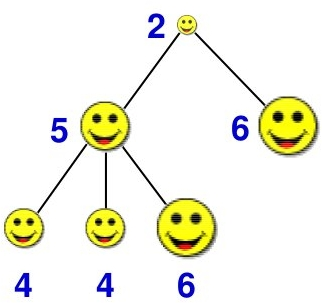
\includegraphics[width=.35\textwidth]{dessins/PartyProblemInput.jpg}
    \quad \quad
    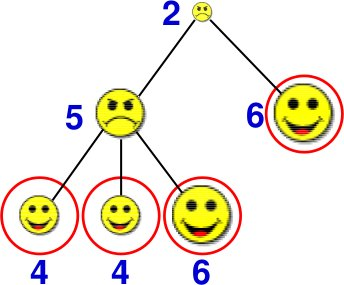
\includegraphics[width=.35\textwidth]{dessins/PartyProblemSolution.jpg}
  \end{center}
  \caption{Instance et Solution du Party Problem}
\end{figure}

\begin{exo}
  Proposer une méthode pour résoudre le problème. Indications.
  \begin{compactitem}
  \item  utiliser une méthode \textsl{bottom-up}; et,
  \item du point de vue d'un sous-arbre de racine v, soit v appartient à la solution
  qu'on veut construire,
  soit v n'appartient pas à cette solution.
  \end{compactitem}
\end{exo}

\paragraph{Notre but.} Le problème de la fête s'appelle (pour des
graphes) \textsc{Maximum weight Independent set}. C'est une généralisation
de \textsc{Independent Set} qui est NP-complet. Or sur un arbre on
vient de voir que ce problème devient polynomial et même \emph{linéaire}. 
Le problème ne devient pas par contre complètement trivial, et on peut
espérer que :
\begin{compactitem}
\item l'approche fonctionne pour d'autres problèmes NP-complets (coloration,
  vertex cover, ...)
\item l'approche fonctionne pour des arbres qui ne sont pas des
  arbres, mais peuvent être décrits par une structure de donnée
  arborescente (notion de largeur arborescente). 
\end{compactitem}


\section{Rappels : définition et exemples décomposition arborescente}




La notion de décomposition arborescente est apparue en théorie des
graphes, au début des années 70. Cette notion a des applications algorithmiques au
niveau théorique (via des résultats très génériques utilisant de la
logique) mais aussi au niveau pratique via des méthodes plutôt
efficaces qui utilisent des techniques de \emph{programmation
  dynamique}). 



\subsection*{Définition informelle}

\

\begin{figure}[h]
  \centering
  \begin{center}
    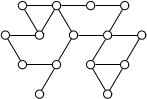
\includegraphics[width=.25\textwidth]{dessins/graphtw.jpg}
    \quad 
    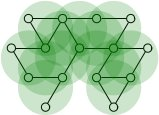
\includegraphics[width=.25\textwidth]{dessins/graphtwbags.jpg}
    \quad 
    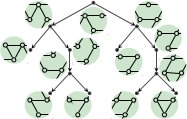
\includegraphics[width=.25\textwidth]{dessins/graphtwtreeofbags.jpg}
  \end{center}
  \caption{Graphe, recouvrement par des sacs, arbre de sacs.}
\end{figure}

\begin{framed}
  \begin{compactitem}
  \item 
    On recouvre le graphe par des petits sacs.
  \item 
    Ces sacs sont les noeuds d'un arbre
  \item 
    Toutes les arêtes sont dans un sac
  \end{compactitem}
  (voir Figure ci-dessus)
  \begin{compactitem}
  \item 
    Pour n'importe quel sac $x$,
    les sacs contenant $x$ forment un sous-arbre. 
  \end{compactitem}
  (voir ci-dessous)
\end{framed}

\begin{figure}[h]
  \centering
  \begin{center}
    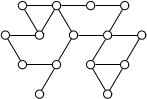
\includegraphics[width=.25\textwidth]{dessins/graphtw.jpg}
    \quad 
    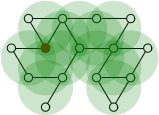
\includegraphics[width=.25\textwidth]{dessins/graphtwbags1vertex.jpg}
    \quad 
    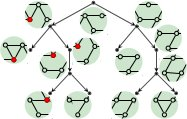
\includegraphics[width=.25\textwidth]{dessins/graphtw1subtree.jpg}
  \end{center}
  \caption{1 sommet correspond à un sous-arbre.}
\end{figure}

\subsection*{Définition formelle}
\label{sec:definition-formelle}

Une \emph{décomposition arborescente} d'un graphe $G$ est un arbre
$\mathcal{T}$ dont les sommets sont des sous-ensembles de sommets de $G$, qu'on
appellera \emph{sacs}, tel que :
\begin{compactitem}
\item Tout sommet du graphe $G$ appartient à un sac
\item Toute arête du graphe $G$ appartient à un sac
\item Pour tout sommet $x$, l'ensemble des sacs contenant $x$ est un
  sous-arbre de $\mathcal{T}$
\end{compactitem}
La largeur de la décomposition est égal au nombre d''éléments du plus
grand sac \emph{moins 1}\footnote{C'est une convention pour que les arbres aient une
  décomposition de largeur 1.}.

\begin{figure}[h]
  \centering
  \begin{center}
    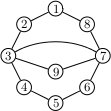
\includegraphics[height=.15\textwidth]{dessins/grapheExoGrohe.jpg}
    \quad 
    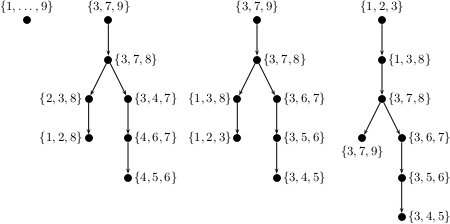
\includegraphics[height=.3\textwidth]{dessins/grapheExoGroheVariousDecompositions.jpg}
  \end{center}
  \caption{Un graphe peut avoir plusieurs décompositions.}
  \label{fig:1graphePlusieursDecomp}
\end{figure}

\begin{exo}
  Montrer que pour un arbre $T$, on peut toujours trouver une
  décomposition de largeur 1.
\end{exo}

\begin{exo}
  Donner une décomposition arborescente de $C_5$ de largeur 3.
\end{exo}

\subsection*{Distance avec un arbre}
\label{sec:distance-avec-un}

La \emph{largeur d'arborescence} d'un graphe $G$ est la largeur minimale
d'une décomposition arborescente de ce graphe, qu'on notera $\tw{G}$
(en anglais, on dit \textsl{the treewidth of} $G$). 

C'est une mesure de la distance à un arbre. Plus le nombre est petit,
plus le graphe ressemble à un arbre.

\begin{exo}
  Quel est la largeur d'arborescence d'un arbre? d'un cycle à $n$
  sommets, $n\geq 3$? d'une clique $K_n$, $n\geq 2$?
\end{exo}

\section{Approfondissement : décomposition arborescente}

\begin{lemma}
  Soient $G$ et $H$ deux graphes. Si $G$ est un mineur de $H$
  (c'est-à-dire qu'on peut l'obtenir par une séquence de contractions d'arêtes,
  suppressions d'arêtes et suppressions de sommets) alors $\tw{G} \leq \tw{H}$.
\end{lemma}

\begin{exo}
  Démontrer le lemme ci-dessus.
  Indication : faites une preuve par récurrence sur le nombre
  d'opérations élémentaires (oubli sommet, oubli arête ou contraction
  d'arête) nécessaires pour construire le mineur; et, transformez une
  décomposition du graphe avant l'opération en une décomposition du
  nouveau graphe.
\end{exo}

\begin{exo}
  Montrer qu'on peut toujours supposer que si $G$ a largeur
  arborescente $k$, alors on peut toujours supposer que $G$ admet une
  \emph{petite décomposition}, c'est-à-dire une décomposition dont
  tous les sacs sont 2 à 2 incomparables pour l'inclusion.
\end{exo}

On comprend maintenant un peu mieux quels graphes sont proches
d'arbres. La question est lesquels sont très différents des arbres. On
verra que les grilles sont un exemple canonique. 

\begin{exo}
  Montrer que un graphe de grille de $n$ lignes et $n$ colonnes
  satisfait $\tw{G}\leq n$.
\end{exo}

\paragraph{Remarque.} 
On peut montrer qu'il n'y a pas de décomposition d'une telle grille de
largeur inférieure à $n$. Pour cela on peut utiliser une
caractérisation en terme de stratégie entre un voleur et des policiers
héliportées (chercher en ligne \textsl{cop and robber game}).

\subsection*{Jeu et largeur arborescente.}
On considère un jeu sur un graphe $G$, paramétré par un entier $k$.
Ce jeu à 2 joueurs oppose $k+1$ gendarmes (joueur I) à un voleur
(joueur II), vus comme des pions que les joueurs vont disposer sur les
sommets du graphe. 
%
Intuitivement, les gendarmes héliportés et peuvent soit voler de
sommet en sommet, soit rester sur un sommet et construire un barrage;
tandis que le voleur est à moto et doit pouvoir s'échapper
indéfiniment en passant d'un sommet à l'autre en traversant les arêtes
du graphe sans passer par un barrage.

Plus précisément.
\begin{compactitem}
\item 
  Au début, le joueur I dispose tous ses gendarmes sur
  les sommets du graphe avec au plus 1 gendarme par sommet; et, le joueur II dispose le voleur sur un
  noeud du graphe où il n'y a pas de gendarme sinon le joueur II perd.
\item 
  Ensuite tant que le joueur II n'a pas perdu (tour $i+1$), 
  le joueur I sélectionne certains gendarmes qu'il dispose ailleurs sur le
  graphe; et, le joueur I déplace ou
  non le voleur sur un sommet accessible dans le graphe depuis sa position
  précédente sans traverser un sommet sur lequel est positionné un
  gendarme n'ayant pas bougé, sinon il perd.
\end{compactitem}

Avec un peu de notation.
\begin{compactitem}
\item \textbf{Tour 0} : I choisit $C_0\subseteq V(G)$ avec $|C_0|=k+1$;
  et, II choisit $r_0 \in V(G) \setminus C_0$ ou perd.
\item \textbf{Tour $i+1$} : I choisit $C_{i+1}\subseteq V(G)$ avec
  $C_{i+1}=k+1$; et, II choisit $r_{i+1} \in V(G)\setminus C_{i+1}$ tel qu'il y ait un
  chemin depuis $r_i$ dont les sommets sont dans $V(G)\setminus (C_i
  \cap C_{i+1})$, sinon il perd.
\end{compactitem}

Le joueur II gagne si il peut s'échapper indéfiniment. 

\begin{lemma}
  Si le joueur I (les gendarmes) a une stratégie gagnante, alors il
  existe une décomposition arborescente du graphe $G$ de largeur $k$.
\end{lemma}
L'intuition de la preuve : celle-ci se fait par récurrence sur le nombre de tours de
jeux maximum avant qu'on attrape le voleur. La condition de début du
jeu fait que c'est clair lorsque il y a 0 tours / une décomposition a
un seul sac $C_0$. Pour la partie récurrente, on applique le résultat à $G\setminus
C_0$. Selon les choix du joueur II pour $r_0$, on obtient par récurrence une
décomposition d'une des composantes connexes de $G\setminus
C_0$ : il suffit de recoller ces décompositions autour du sac $C_0$.

\begin{wrapfigure}[11]{r}{0.4\textwidth}
  \vspace{-30pt}
  \begin{center}
    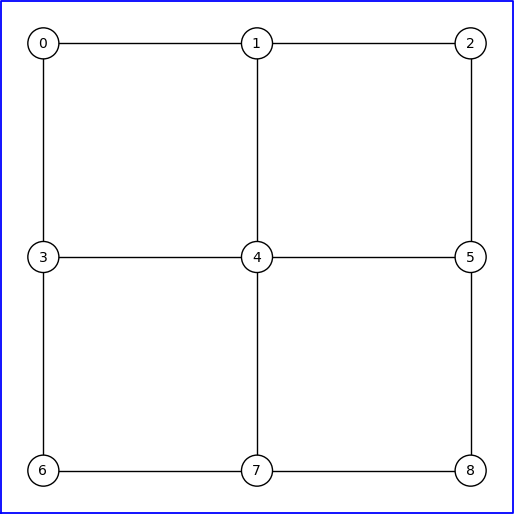
\includegraphics[width=0.39\textwidth]{dessins/DevoirExo3JeuGrille3x3.png}
  \end{center}
  \vspace{-30pt}
\end{wrapfigure}
\paragraph{Question 1.} Montrez l'implication inverse, à savoir si il existe une décomposition
arborescente du graphe $G$ de largeur $k$ alors le joueur I (les
gendarmes) a une stratégie gagnante.
\paragraph{Question 2.} On considère le graphe d'une grille $3\times 3$ (voir figure ci-contre). Montrez que le joueur
II (le voleur) a un stratégie gagnante dans le jeu qui l'oppose à
$k+1=3$ gendarmes.
\paragraph{Question 3.} Expliquer sans rentrer dans les détails comment calculer qui des
policiers ou du voleur a une stratégie gagnante (vous pouvez vous
appuyez sur un cas concret, en esquissant par exemple une partie du calcul
pour la grille $3\times 3$). 


%%%%%%%%%%%%%%%%%%%%%%%%%%%%%%%%%%%%%%%%%%%%%%%%%%%%%%%%%%%%%%%%%%

\subsection*{Décompositions gentilles}
Il sera pratique pour le design d'algorithmes / preuve de leur
fonctionnement correct de travailler sur ces décompositions particulières.

Il s'agit de décompositions qui sont enracinées ayant 4 sortes de sacs :
\begin{compactitem}
\item Les sacs feuilles contenant un seul élément;
\item Les sacs oublis ont pour unique descendant un sac ayant exactement un
  élément de moins;
\item Les sacs ajouts ont pour unique descendant un sac ayant
  exactement un élément de plus; et,
\item Les sacs de jointure ayant exactement 2 descendants, tous deux
  ayant les mêmes éléments.
\end{compactitem}
\begin{figure}[h]
  \centering
  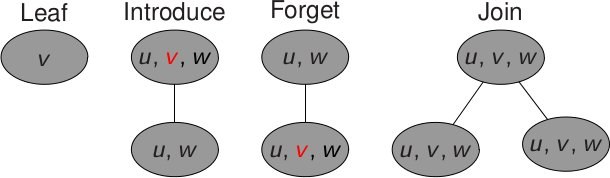
\includegraphics[width=.7\textwidth]{dessins/NiceDecompositions.jpg}
  \caption{Les 4 types de noeuds d'un arbre d'une décomposition gentille.}
\end{figure}
\begin{exo}
  Montrer qu'on peut construire à partir d'une décomposition $\mathcal{T}$ de
  largeur $k$ d'un graphe $G$ à $n$ sommets une gentille décomposition $\mathcal{T}'$
  de largeur $k$ ayant au plus $O(k.n)$ sommets (sacs).
  %Correction. 
  % On commence par faire en sorte que 2 sacs voisins diffèrent d'au
  % plus 1 élément.
  % Si 2 sacs voisins avec $\{x1,x2,\ldots,xl\}$ en commun,
  %$\{x1,x2,\ldots,xl,x_{l+1},\ldots,x_{k'}\}$ et $\{x1,x2,\ldots,xl,y_{l+1},\ldots,y_{k''}\}$ 
  %avec $l<k',k'' \leq k$.
  %remplacer par chemin avec ajout de nouveaux sacs :
  %Une séquence d'oublis : $\{x1,x2,\ldots,xl,x_{l+1},\ldots,x_{k'}\}$
  %puis $\{x1,x2,\ldots,xl,x_{l+1},\ldots,x_{k'-1}\}$ etc jusqu'à
  %$\{x1,x2,\ldots,xl\}$
  % suivi d'une séquence d'ajouts
  %$\{x1,x2,\ldots,xl,y_{l+1}\}$ etc jusqu'à
  %$\{x1,x2,\ldots,xl,y_{l+1},\ldots,y_{k''}\}$.
  %Ensuite on peut avoir des sommets ayant des degrés sortant
  %arbitraires.
  % On les duplique à l'aide de noeuds join.
  % 
\end{exo}

\subsection*{Extension de notre exemple}
\label{sec:extension-de-notre}

Reprenons l'exemple du \emph{party problem}, formellement il s'agit de
trouver un ensemble indépendant de poids maximal d'un graphe. Cette
fois, on dépasse l'organisation hiérarchique purement arborescente, et
on considère des organisations plus réalistes : on suppose que cet
organigramme peut être représenté par un graphe ayant une
décomposition arborescente de petite largeur $k$. 

\begin{exo}
  On considère comme instance le graphe de la
  figure~\ref{fig:1graphePlusieursDecomp}, dont les poids seront égaux
  au numéro du sommet plus votre âge modulo 3.

  \begin{itemize}
  \item 
    Calculez un ensemble indépendant de poids maximal pour cette instance.
  \item 
    Recommencez en vous appuyant sur une décomposition.
    Remarque : on
    peut essayer de rendre les décompositions plus simples à manipuler
    quitte à avoir un arbre de décomposition un peu plus grand, voir
    la section précédente sur les décompositions gentilles (vous n'êtes pas
    obligés d'aller jusqu'à l'étape qui ajoute des feuilles)
  \end{itemize}
\end{exo}


\section{Algorithmes utilisant la décomposition}

\subsection*{Un autre exemple : la colorabilité}
\label{sec:un-autre-exemple}

%On considère le problème de décision suivant.
\begin{framed}\textsc{$\ell$-col For Tree decompositions}
  \begin{compactitem}
  \item \textbf{paramètre}: $k$
  \item \textbf{instance}: $G$ et une décomposition arborescente de
    $G$ de largeur au plus $k$.
  \item \textbf{question}: Est-ce-que $G$ est $\ell$-colorable? 
  \end{compactitem}
\end{framed}

\begin{exo}
  Montrez que ce problème est polynomial en la taille du graphe
  d'entrée $n$ et exponentiel en $k$.

  Indication : inspirez vous du travail sur le party problem et son
  extension (maximum weighted independent set); utilisez une approche
  \textsl{bottom-up} en trouvant la bonne quantité d'information à
  stocker/calculer sur chaque noeud de l'arbre.
\end{exo}

% \subsection*{Un autre exemple : \textsl{vertex cover}}

% %On considère le problème de décision suivant.
% \begin{framed}\textsc{Vertex Cover For Tree decompositions}
%   \begin{compactitem}
%   \item \textbf{paramètre}: $k$
%   \item \textbf{instance}: $G$ et une décomposition arborescente de
%     $G$ de largeur au plus $k$.
%   \item \textbf{output}: un vertex cover de taille minimale 
%   \end{compactitem}
% \end{framed}

% \begin{exo}
%   Montrez que ce problème est polynomial en la taille du graphe
%   d'entrée $n$ et exponentiel en $k$.
% \end{exo}

\subsection*{Et l'énumération dans tout ça?}

\begin{exo}
  Reprendre les problèmes de la question précédentes mais cette fois
  en considérant la version énumérative du problème.
  C'est-à-dire pour des prédicats $R$ de $I\times O$ où $I$ consiste
  en l'ensemble des paires un graphe et sa décomposition de largeur
  bornée par $k$ et $O$ consiste en l'ensemble des solutions
  correspondants au problème étudié ($\ell$-coloriage ou vertex cover
  minimal). 

  Quel délai pouvez vous garantir entre 2 solutions?
\end{exo}

%\pagebreak

\section{Pour quels problème peut-on toujours utiliser la décomposition?}
\label{sec:TractableBtwMSO}

\subsection*{Tout NP?}
On peut se poser la question naturelle de la limite de cette
approche. En particulier, \emph{peut-on prendre n'importe quel problème de NP et garantir que ce
problème devient polynomial si on a une décomposition arborescente de
largeur bornée?}

\paragraph{Non.} Ce n'est pas vrai par exemple pour \textsc{Edge-disjoint paths}
%Nishizeki,Vygen,Zhou'01
(NP-complet pour une largeur de $2$)
ou encore 
pour \textsc{Weighted $\ell$-coloring} (NP-complet pour une largeur de
$3$).
%(McDiarmid & Reed ’01)

Ces problèmes sont définis ci-dessous.
\begin{framed}\textsc{Edge Disjoint Paths With
  Tree Decomposition}
  \begin{compactitem}
  \item \textbf{paramètre} : $k$
  \item \textbf{instance} : un graphe $G$, une décomposition de
    largeur au plus $k$, et $\ell$ paires de sommets distincts $s_i,t_i$.
  \item \textbf{question} : peut-on trouver des chemins de $s_i$ à
    $t_i$ qui soient disjoints 2-à-2 
    pour les arêtes?
  \end{compactitem}
\end{framed}

\begin{framed}
  \textsc{Weighted $\ell$-coloring With
  Tree Decomposition}
  \begin{compactitem}
  \item \textbf{paramètre} : $k$
  \item \textbf{instance} : un graphe $G$, une décomposition de
    largeur au plus $k$, et une fonction de poids sur les arêtes de
    $G$ $w:E(G) \to \{1,2,\ldots,\ell\}$
  \item \textbf{question} : peut-on trouver une fonction $c:V(G)\to
    \{1,2,\ldots,\ell\}$ telle que pour toute arête $e=\{x,y\}$ de
    $E(G)$ on a $|c(u)-c(v)|\geq w(e)$?
  \end{compactitem}
\end{framed}

\subsection*{Méthode OK pour MSO}
On voudrait donc comprendre \emph{pour quels problème de NP notre méthode
\emph{bottom-up} s'applique?} Évidemment, on pourrait lister de nombreux problèmes et
pour chacun d'eux chercher à adapter notre approche. Il existe
toutefois un résultat très général qui permet de montrer que beaucoup
de problèmes deviennent polynomiaux lorsque on les donne via une
décomposition arborescente. Ce résultat fait intervenir une logique
qu'on appelle \emph{la logique Monadique du second ordre} (MSO) pour faire
court. Dans l'immédiat, vous pouvez imaginer MSO comme une sorte de
langage de programmation plutôt riche bien qu'il ne permet pas de programmer absolument ce
qu'on veut et dont les programmes peuvent tous être exécutés en espace
polynomial (dans la classe de complexité Pspace).
Ce langage permet d'exprimer des propriétés sur les graphes qui
parlent d'ensembles de sommets ou d'arêtes.

\begin{theorem}[Courcelle]
  Soit $k$ une constante fixée.
  Tout problème MSO est polynomial lorsque l'entrée $G$ est
  accompagnée d'une décomposition de largeur au plus $k$.
\end{theorem}

%%% TO DO? check
% \paragraph*{Remarque.} La classe des problème qu'on peut exprimer en
% MSO est incomparable avec NP. Il y a des problèmes de NP qu'on ne peut
% pas exprimer avec MSO.
% all conjecture?

\paragraph*{C'est quoi MSO?}
Ce langage généralise \emph{la logique du premier ordre}, c'est-à-dire
les formules qu'on peut écrire à l'aide des quantificateurs
existentiels ($\exists$) et universels ($\forall$) qui porteront sur
des variables qui sont des sommets du graphe d'entrée, des connecteurs
logiques usuels conjonction ($\land$) disjonction ($\lor$) et négation
($\lnot$) et donc tous les connecteurs qu'on peut simuler ($\implies$,
$\iff$, xor ...), et des tests sur les arêtes du graphe (on écrira
$E(x,y)$ pour dire qu'il y a une arête entre $x$ et $y$).

On peut voir la logique du premier ordre comme un langage de
programmation permettant d'écrire des tests vérifiant 
des conditions locales sur le graphe d'entrée pour certains sommets ou
arêtes. Par exemple, ``il existe un triangle dans mon graphe'' ou
encore ``il existe un sommet $x$ qui est voisin de tous les autres
sommets'' ou encore ``il existe 42 sommets tels que toute arête du
graphe est incidente à un de ces 42 sommets''
Par contre, on ne peut pas exprimer des choses plus globales comme
``mon graphe est connexe'' mais on peut dire des choses bornées comme
``mon graphe a un diamètre de 321 ou moins'' en écrivant quelque chose comme
``Pour toute paire de sommets $x$ et $y$, il existe 320 autres sommets qui forment
un chemin de $x$ à $y$ ou il existe 319 sommets qui forment un chemin
de $x$ à $y$ ou ... ou $x$ et $y$ sont voisins ou ils sont égaux''.

Pour pallier à cette faiblesse, on peut ajouter des quantificateurs
qui portent sur des ensembles de sommets ou des ensembles
d'arêtes\footnotemark{}.
\footnotetext{Dans la littérature, on fait une distinction fine entre
  le cas où on ne peut pas quantifier sur les ensembles d'arêtes qui
  est noté MSO1 et le cas plus général qu'on considère ici qui est
  noté par MSO2.}
Dans le jargon, on ne dit pas ``quantificateur sur un ensemble'' mais
``quantificateur sur un prédicat monadique''. On obtient ainsi la
fameuse \emph{logique monadique du second ordre}\footnotemark{} qu'on notera par MSO.
\footnotetext{Ici le \emph{second} ordre veut dire qu'on a des
  quantificateurs sur des choses qui ne sont pas des éléments du
  graphe, mais plus généralement des relations entre ces éléments.}
On peut alors exprimer des choses plus globales comme ``mon graphe
n'est pas un arbre'' puisqu'on peut exprimer que ``mon graphe contient
un cycle'' de la manière suivante.

\begin{verbatim}
Il existe un sous-ensemble de sommets C                // MONADIQUE EXISTENTIEL
tel que
Il existe au moins 1 élément dans C                   // SUITE DU PREMIER ORDRE
et
Tout sommet v de C a au moins 2 voisins distincts eux aussi dans C.
\end{verbatim}

Comme vous pouvez le voir avec l'exemple ci-dessus, ce n'est pas
forcément un langage très facile à manipuler sans entraînement. Par
contre, comme dans un langage de programmation classique, on peut
avoir une approche modulaire et écrire informellement 
\begin{verbatim}
Il existe un ensemble d'arêtes C formant un arbre
\end{verbatim}
comme abréviation pour la formule précédente.

Comme autre exemple, on peut exprimer qu'un graphe n'est pas connexe
(chose qu'on ne peut pas exprimer avec la logique du premier ordre).
\begin{verbatim}
Il existe 2 sommets distincts x,y
Il existe un sous ensemble de sommets Cx               // MONADIQUE EXISTENTIEL
tel que
Cx contient x
Cx ne contient pas y 
Pour tout sommets adjacents y et z
y appartient à Cx
ssi
z appartient à Cy 
\end{verbatim}
On peut donc, même sans expérience, se munir d'une boîte à outil MSO permettant de mieux
cerner ce qu'on peut exprimer en MSO, de même qu'un programmeur n'a
pas nécessairement besoin de savoir implanter les fonctions d'une
librairie qu'il appelle.
 
On peut très facilement exprimer des coloriages, des partitions, en
particulier sur les sommets. 
\begin{exo}
  Décrire informellement un programme MSO pour exprimer qu'un graphe
  est 3 colorable.
\end{exo}

\begin{exo}
  Adaptez le ``programme'' MSO ci-dessus pour exprimer que H (un
  ensemble d'arêtes) forme un \emph{arbre couvrant} du graphe en entrée. 
\end{exo}

\paragraph{Remarque.} Une limite de MSO est qu'on ne peut pas compter. En fait on ne peut
même pas compter modulo 2 : il n'existe pas de
formule MSO permettant d'exprimer que le graphe a un nombre pair de
sommets. 

\subsection*{Un résultat plus général.} 
En fait le théorème de Courcelle
est beaucoup plus général que le 
résultat ci-dessus. Il s'agit d'une version uniforme du résultat
ci-dessus. Il existe un algorithme  qui prend 
en entrée, à la fois la formule MSO $\varphi$ (comprendre le programme
MSO), le graphe sur
lequel on veut l'appliquer $G$ et une décomposition et donne en sortie
la réponse à la question "est-ce-que $G$ satisfait le problème exprimé
par $\varphi$?". Cet algorithme qu'on peut intuitivement voir comme une sorte de compilateur
MSO / run-time sur graphes de largeur bornée fonctionne en temps 
$O(f|\varphi|+ 2^{p(tw(G))}. |G|)$, où $f$ est une fonction sur les
entiers qui est calculable, $p$ est un polynôme et $|\varphi|$ et
$|G|$ représente la taille de $\varphi$ et $G$ respectivement. 

\paragraph{\textsl{Happy end?}}
Si on examine plus en détails ce résultat il y a des choses très
positives lorsque le problème MSO est fixé (ce qui sera notre cas) :
on obtient un algorithme qui est FPT (\emph{fixed parameter
  tractable}) c'est-à-dire où le paramètre est indépendant de la
taille $n$ de l'entrée. Intuitivement : la difficulté n'est pas
vraiment dans le parcours de l'arbre de décomposition mais isolé dans
le calcul associé à chaque sac et pour
recoller les morceaux de calculs des fils vers leur père. Cela veut
dire que pour un graphe énorme, tant que les sacs ne sont pas trop
gros (= ce que vous pouvez vous permettre avec votre ressource de
calcul), votre algorithme est applicable.

\paragraph{Non pas vraiment.}
Il y a par contre une difficulté cachée dans la constante additive
$f(k)$, où $f$ est une fonction calculable. Cette fonction croît très
vite et donnera des \emph{constantes impraticables} pour des programmes
complexes. La preuve de Courcelle repose sur la construction
d'automates d'arbres et en particulier l'alternance des
quantificateurs donneront lieu à des tours d'exponentielles.

\paragraph{Synthèse.} Si le nombre d'alternances de quantificateurs est
restreint, on peut tout de même obtenir un prototype pour un problème avec des
outils de logique / combinatoire. Ceci reste sans grand intérêt
pratique mais permet immédiatement de savoir que l'approche via la
décomposition arborescente est théoriquement possible. Ensuite
survient un travail pratique d'élaboration d'un algo concret pour le
problème qu'on étudie.  

\section{Calculer une décomposition arborescente}

Ce problème est NP-complet.

\begin{framed}\textsc{Tree-Width}
  \begin{compactitem}
  %\item \textbf{parameter}:
  \item \textbf{instance} : un graphe $G$, un entier $k$
  \item \textbf{question} : est-ce-que $\tw{G}\leq k$? 
  \end{compactitem}
\end{framed}

Par contre celui-ci est polynomial.
\begin{framed}\textsc{Parameterised Tree-Width}
  \begin{compactitem}
  \item \textbf{paramètre} : $k$
  \item \textbf{instance} : un graphe $G$
  \item \textbf{question} : est-ce-que $\tw{G}\leq k$? 
  \end{compactitem}
\end{framed}

En fait il existe un algorithme dû à Bodlaender qui étant donné un
graphe $G$ calcule une décomposition de largeur optimal (égale à
$\tw{G}$) en temps $O(2^{p(\tw{G})}.|G|)$, où $p$ est un polynôme de
degré 3.

Ceci montre que le problème est FPT dans sa version paramétrée. 
% \footnotetext{\textsl{Fixed Parameter Tractable} : classe de
%   complexité paramétrée c'est-à-dire à 2 dimensions, l'entrée $n$ et le paramètre
%   $k$, où la complexité en temps est de l'ordre $f(k).p(n)$ où $f$
%   peut-être une fonction hyper-croissante (e, fait n'importe quelle
%   fonction calculable), mais $p$ est un polynôme.}
En pratique, toutefois cette dépendance en $2^{(k^3)}$ limite vraiment
la grandeur du paramètre $k$ pour lesquels on peut se permettre de
calculer exactement une décomposition. 

Une approche alternative consiste à utiliser un autre algorithme  basé
sur les séparateurs qui lui est en $O(2^{3.\tw{G}}.\tw{G}.|G|^2)$. 
Ce second algorithme ne calcule pas une décomposition de largeur $k$
mais une approximation (décomposition de largeur $3k+2$). Finalement,
il existe des heuristiques permettant de décomposer les graphes, mais
sans garantie d'exécution en temps polynomial.

\paragraph{Conséquence}
Tous les problèmes de ce cours où j'ai écrit pour l'instance un graphe
et sa décomposition et pour paramètre sa largeur restent FPT \emph{si on ne donne
  pas la décomposition}. On calcule par exemple une approximation de sa
décomposition en temps $O(2^{3.\tw{G}}.\tw{G}.|G|^2)$, c'est-à-dire
une décomposition de largeur au plus $3k+2$ puis on applique la
méthode bottom-up associée au problème qui fonctionne en temps
exponentiel en la taille des sacs pour chaque sac (ici $3k+2$) lors du
traitement d'un sac, multiplié par la taille de l'arbre de
décomposition (qui est linéaire en la taille du graphe). 
Par exemple, pour la 3 colorabilité qui est naïvement en
$3^{\text{nbre de sommets}}$, on obtient un temps total de la forme
$O(2^{3.\tw{G}}.\tw{G}.|G|^2 + 3^{(3k+2)}.|G|)$.

Dans une perspective pratique, il faudra étudier expérimentalement
différentes implantations selon les instances typiques qu'on veut
résoudre : il sera alors plus ou moins intéressant de travailler sur
des décompositions de largeur très proche de $\tw{G}$ ou non.

\section{Pour aller plus loin}
Je vous invite à découvrir la logique monadique dans les premiers
chapitres du livre de Courcelle et Engelfriet~\cite{DBLP:books/daglib/0030804} (je peux vous aider à trouver une version de prépublication
gratuite en ligne). Le livre de Flum et grohe~\cite{FlumGrohe2006} sur
la complexité paramétrée vous en apprendra plus sur le sujet, en
particulier le chapitre 11 sur les décompositions arborescentes, et
comment on les calcule (je peux vous aider à trouver une version
gratuite de ce chapitre 11).

\nocite{*}
\bibliographystyle{plain}
\bibliography{biblio}

\section*{Sources}
De nombreuses figures de ce script ont été glané sur divers cours
disponible sur internet dans des documents mis à disposition par Daniel Marx,
Martin Grohe et Michael Elberfeld.

\end{document}

%%%%%%%%%%%%%%%%%%%%%%%%%%
%\tableofcontents{}

\newpage

\begin{center}
  \LARGE \textbf{Devoir à la maison}\\
  \large à rendre pour le 9 janvier \\
  \large une soutenance \emph{individuelle} de 5 à 10 minutes
  organisée ultérieurement permettra de juger de la compréhension de
  ce que chaque étudiant a rendu
\end{center}
\section*{Exo 1 (polynôme chromatique)}
On admettra que le graphe ci-dessous a pour polynôme chromatique
$(x - 2) \cdot x \cdot (x - 1)^{2} \cdot (x^{2} - 3x + 3)$
\begin{center}
  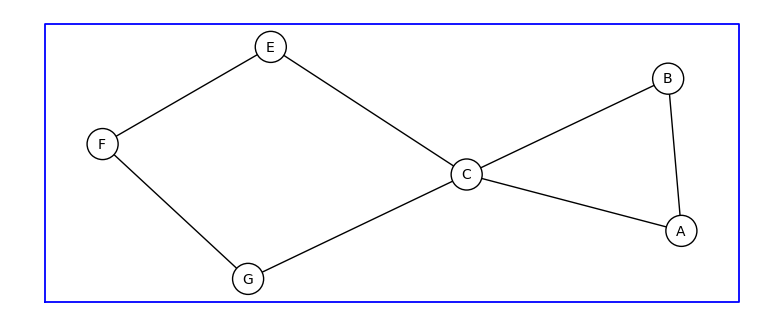
\includegraphics[height=5cm]{dessins/DevoirExo1Fish.png}
\end{center}

En déduire que le polynôme chromatique du graphe ci-dessous est
$$(x - 2)^{2} \cdot x^{3} \cdot (x - 1)^{7} \cdot (x^{2} - 3x + 3)^{2}$$

\begin{center}
  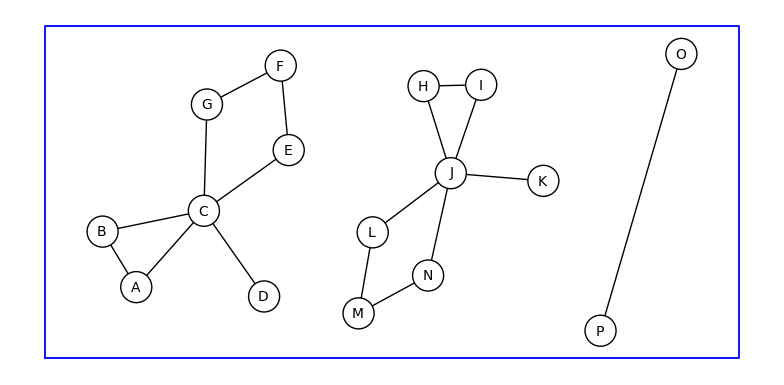
\includegraphics[height=7cm]{dessins/DevoirExo1PolChrom.png}
\end{center}

\textbf{Indications} : on pourra utiliser une méthode proche de celle vue en
cours et étudiée en exercice qui relie polynôme chromatique d'un
graphe ayant une arête $x,y$ avec celui du graphe obtenu en enlevant
cette arête et en la contractant, respectivement.



%%% Correction.
%%% le polynome chromatique étant le produit des polynomes de chaque
%%% composante connexe, et comme on sait que P2 a pour pol chrom
%%% $x(x-1)$, on peut diviser la quantité à trouver par cette valeur
%%% et ne considérer que le graphe induit par les sommets de A à N. 
%%% Pour ce graphe on doit trouver
%%% $$(x - 2)^{2} \cdot x^{\mathbf{2}} \cdot (x - 1)^{\mathbf{6}} \cdot (x^{2} - 3x + 3)^{2}$$
%%% En regardant attentivement les 2 autres composantes connexes, on
%%% s'aperçoit qu'elles sont isomorphes. Il suffit donc de prendre la
%%% racine du polynôme ci-dessus, ce qui donne
%%% $$(x - 2) \cdot x \cdot (x - 1)^{\mathbf{3}} \cdot (x^{2} - 3x + 3)$$
%%% et de montrer qu'il s'agit bien du polynôme chromatique du graphe
%%% induit par les sommets de A à G.
 
\pagebreak
\section*{Exo 2 (décomposition arborescente)}
Donnez une décomposition arborescente de largeur minimale pour le graphe
ci-dessous, en expliquant bien pourquoi elle est minimale.
\begin{center}
  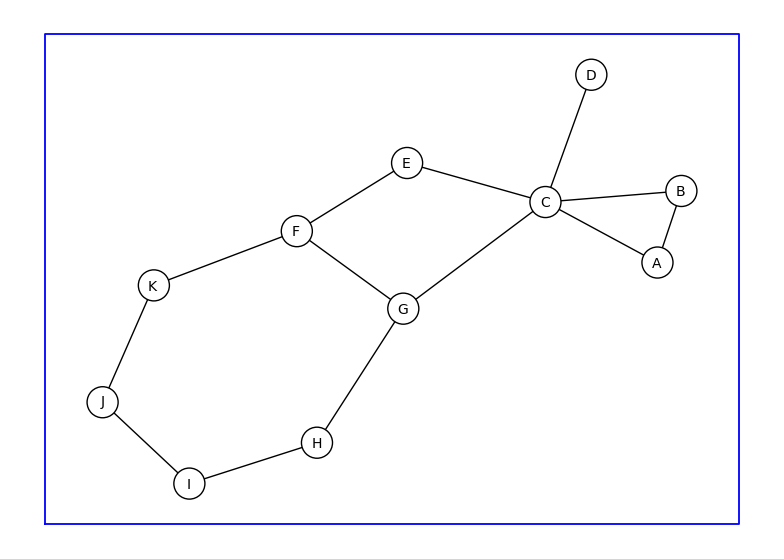
\includegraphics[width=.8\textwidth]{dessins/DevoirExo2Decomposition.png}
\end{center}

\pagebreak
\section*{Exo 3 (jeu et largeur arborescente)}
On considère un jeu sur un graphe $G$, paramétré par un entier $k$.
Ce jeu à 2 joueurs oppose $k+1$ gendarmes (joueur I) à un voleur
(joueur II), vus comme des pions que les joueurs vont disposer sur les
sommets du graphe. 
%
Intuitivement, les gendarmes héliportés et peuvent soit voler de
sommet en sommet, soit rester sur un sommet et construire un barrage;
tandis que le voleur est à moto et doit pouvoir s'échapper
indéfiniment en passant d'un sommet à l'autre en traversant les arêtes
du graphe sans passer par un barrage.

Plus précisément.
\begin{compactitem}
\item 
  Au début, le joueur I dispose tous ses gendarmes sur
  les sommets du graphe avec au plus 1 gendarme par sommet; et, le joueur II dispose le voleur sur un
  noeud du graphe où il n'y a pas de gendarme sinon le joueur II perd.
\item 
  Ensuite tant que le joueur II n'a pas perdu (tour $i+1$), 
  le joueur I sélectionne certains gendarmes qu'il dispose ailleurs sur le
  graphe; et, le joueur I déplace ou
  non le voleur sur un sommet accessible dans le graphe depuis sa position
  précédente sans traverser un sommet sur lequel est positionné un
  gendarme n'ayant pas bougé, sinon il perd.
\end{compactitem}

Avec un peu de notation.
\begin{compactitem}
\item \textbf{Tour 0} : I choisit $C_0\subseteq V(G)$ avec $|C_0|=k+1$;
  et, II choisit $r_0 \in V(G) \setminus C_0$ ou perd.
\item \textbf{Tour $i+1$} : I choisit $C_{i+1}\subseteq V(G)$ avec
  $C_{i+1}=k+1$; et, II choisit $r_{i+1} \in V(G)\setminus C_{i+1}$ tel qu'il y ait un
  chemin depuis $r_i$ dont les sommets sont dans $V(G)\setminus (C_i
  \cap C_{i+1})$, sinon il perd.
\end{compactitem}

Le joueur II gagne si il peut s'échapper indéfiniment. 

On admettra le lemme suivant.
\begin{lemma}
  Si le joueur I (les gendarmes) a une stratégie gagnante, alors il
  existe une décomposition arborescente du graphe $G$ de largeur $k$.
\end{lemma}

\begin{wrapfigure}[11]{r}{0.4\textwidth}
  \vspace{-30pt}
  \begin{center}
    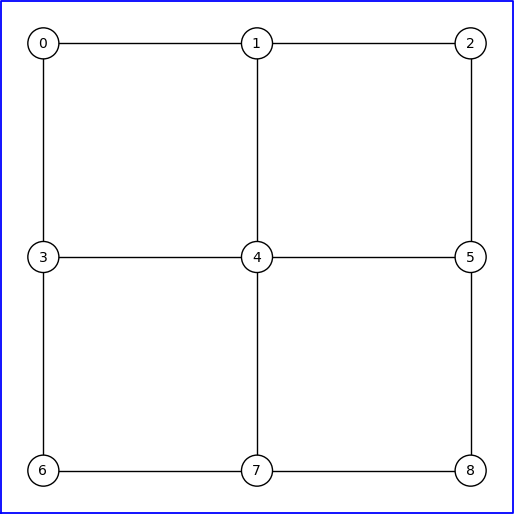
\includegraphics[width=0.39\textwidth]{dessins/DevoirExo3JeuGrille3x3.png}
  \end{center}
  \vspace{-30pt}
\end{wrapfigure}
\paragraph{Question 1.} Montrez l'implication inverse, à savoir si il existe une décomposition
arborescente du graphe $G$ de largeur $k$ alors le joueur I (les
gendarmes) a une stratégie gagnante.
\paragraph{Question 2.} On considère le graphe d'une grille $3\times 3$ (voir figure ci-contre). Montrez que le joueur
II (le voleur) a un stratégie gagnante dans le jeu qui l'oppose à
$k+1=3$ gendarmes.
\paragraph{Question 3.} Expliquer sans rentrer dans les détails comment calculer qui des
policiers ou du voleur a une stratégie gagnante (vous pouvez vous
appuyez sur un cas concret, en esquissant par exemple une partie du calcul
pour la grille $3\times 3$). 

\pagebreak
\section*{Exo 4 (programmation dynamique)}
On considère le problème combinatoire de 3-colorabilité.
Programmer la méthode \textsl{bottom-up} vue en cours prenant en
entrée un graphe $G$ et une décomposition arborescente, permettant
selon les désirs de l'utilisateur de décider, générer une solution,
compter les solutions ou énumérer les solutions.

Pour tester votre programme, voici 2 instances (graphe +
décomposition).

\paragraph{Instance 1.}
\begin{center}
  \begin{minipage}[h]{\linewidth}
    \begin{minipage}[h]{.5\linewidth}
      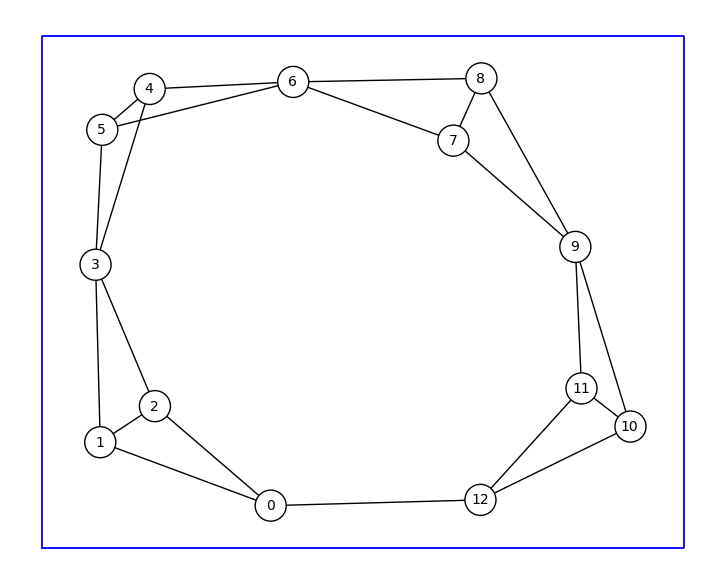
\includegraphics[height=7cm]{dessins/DevoirExo4ColDecompNoInstance.png}
    \end{minipage}
    \quad
    \quad
    \begin{minipage}[h]{.15\linewidth}
      
\includegraphics[height=6cm]{dessins/DevoirExo4ColDecompNoInstanceDecomp.png}
    \end{minipage}
    %\quad
    \begin{minipage}[h]{.2\linewidth}
      Avec les sacs : \\
      
      $
      \begin{array}[h]{l}
        A : \{0,1,2,3\}\\
        B : \{0,3,4,5\}\\
        C : \{0,4,5,6\}\\
        D : \{0,6,7,8\}\\
        E : \{0,7,8,9\}\\
        F : \{0,9,10,11\}\\
        G : \{0,10,11,12\}\\
      \end{array}
      $
    \end{minipage}
  \end{minipage}
\end{center}

\paragraph{Instance 2.}
\begin{center}
  \begin{minipage}[h]{\linewidth}
    \begin{minipage}[h]{.5\linewidth}
      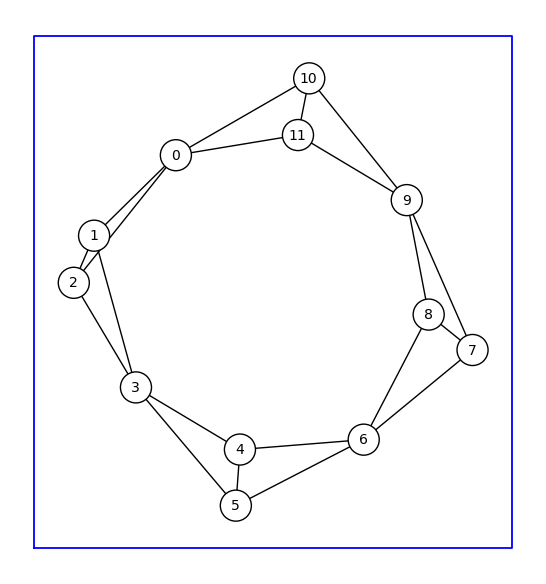
\includegraphics[height=7cm]{dessins/DevoirExo4ColDecompYesInstance.png}
    \end{minipage}
    \quad
    \quad
    \begin{minipage}[h]{.15\linewidth}
      
\includegraphics[height=6cm]{dessins/DevoirExo4ColDecompYesInstanceDecomp.png}
    \end{minipage}
    %\quad
    \begin{minipage}[h]{.2\linewidth}
      Avec les sacs : \\

      $
      \begin{array}[h]{l}
        A : \{0,1,2,3\}\\
        B : \{0,3,4,5\}\\
        C : \{0,4,5,6\}\\
        D : \{0,6,7,8\}\\
        E : \{0,7,8,9\}\\
        F : \{0,9,10,11\}\\
      \end{array}
      $
    \end{minipage}
  \end{minipage}
\end{center}

\end{document}

%%% Local Variables: 
%%% mode: latex
%%% TeX-master: t
%%% End: 

%%%%%%%%% Problème
\begin{framed}\textsc{Titre}
  \begin{compactitem}
  \item \textbf{parameter}:
  \item \textbf{instance}:
  \item \textbf{question}:
  \end{compactitem}
\end{framed}


\grid
